\chapter{STRique Repeat Detection}
\label{sec:strique}

Expansions of short tandem repeats are genetic variants that have been implicated in several neuropsychiatric and other disorders, but their assessment remains challenging with current polymerase-based methods. Here we introduce a CRISPR–Cas-based enrichment strategy for nanopore sequencing combined with an algorithm for raw signal analysis. Our method, termed STRique for short tandem repeat identification, quantification and evaluation, integrates conventional sequence mapping of nanopore reads with raw signal alignment for the localization of repeat boundaries and a hidden Markov model-based repeat counting mechanism. We demonstrate the precise quantification of repeat numbers in conjunction with the determination of CpG methylation states in the repeat expansion and in adjacent regions at the single-molecule level without amplification. Our method enables the study of previously inaccessible genomic regions and their epigenetic marks.

\begin{figure}[h]
    \centering
    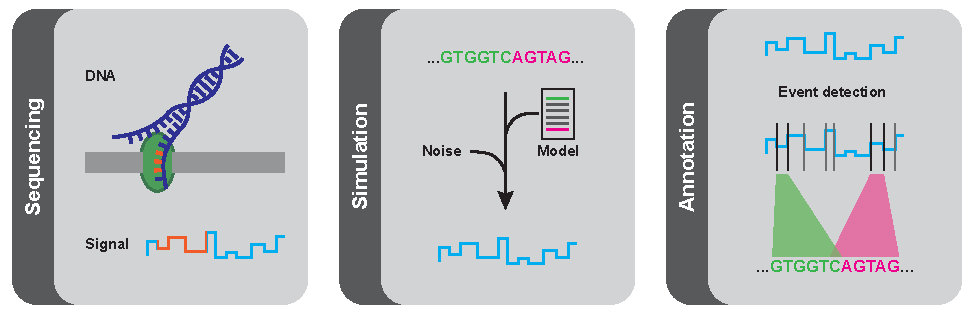
\includegraphics[width=1.0\textwidth]{figures/strique/GA.pdf}
    \label{fig:strique:ga}
\end{figure}


\section{Background}
\label{sec:strique:background}

\section{Data Generation}
\label{sec:strique:data}

\section{Repeat Quantification}
\label{sec:strique:quantification}

\section{Base Modification Detection}
\label{sec:strique:modifications}

\section{Summary}
\label{sec:strique:summary}
